\section{Results and Discussion}\label{sec:Discussion}

\subsection{Logistic Regression}

Logistic regression was employed using both $L_1$ and $L_2$ regularization. The space over the regularization parameters
was searched under bootstrapping to explore the consequence on bias and variance. The results are shown in~\cref{fig:logreg} and~\cref{fig:logregl1}.

The usual pattern is observed. Increasing the regularization strength initially
reduces the error by decreasing the variance, but too high a regularization shrinks
the solution space sufficiently such that the bias skyrockets. The change is most dramatic for $L_1$ as many predictors are set to $0$.

\begin{figure}[H]
    \centering
    \begin{subfigure}
        \centering
        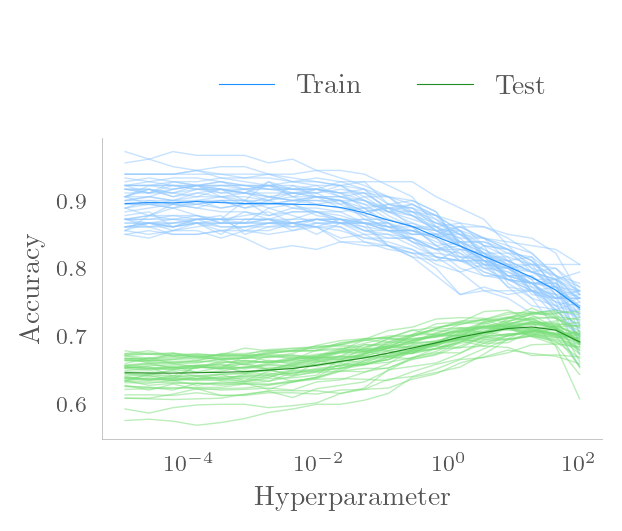
\includegraphics{Figures/logreg_bootstrap.png}
        \caption{The accuracy for different bootstrap samples of training and
        test data.}
    \end{subfigure}
    \begin{subfigure}
        \centering 
        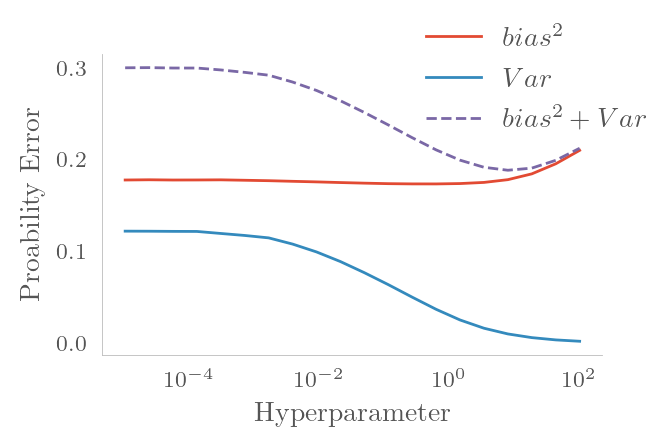
\includegraphics{Figures/logreg_biasvar.png}
        \caption{The error in predicted probability decomposed as bias squared and variance. }
    \end{subfigure}
    \caption{The quality of classification as function of $L_2$ regularization
    hyperparameter. Increasing the regularization prevents overfitting by decreasing variance, increasing the test accuracy. A too high regularization ($>1$) causes
    an increase in bias, deteriorating the accuracy.}
    \label{fig:logreg}
\end{figure}

\begin{figure}[H]
    \centering
    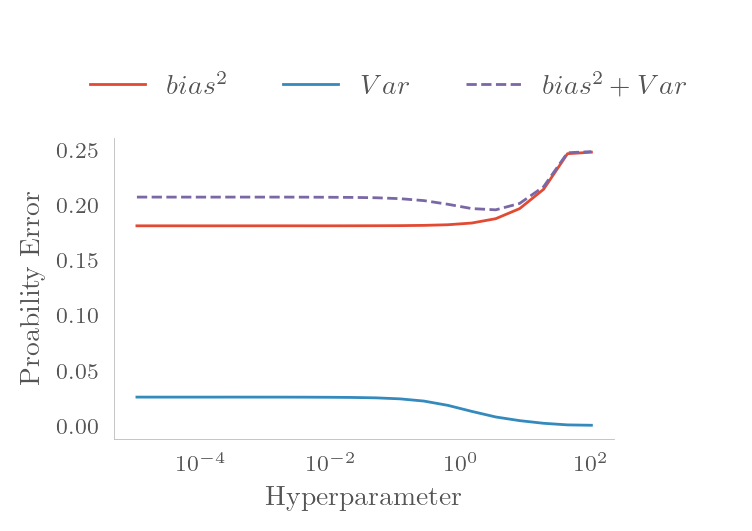
\includegraphics{Figures/logreg_biasvar_l1.png}
    \caption{The decomposition of error as a function of $L_1$ regularization
    strength. The error changes slightly after $>10^{-1}$ by decreasing the variance, but quickly jumps as bias grows at an increasing rate.}
    \label{fig:logregl1}
\end{figure}

As $L_2$ and $L_1$ give practically identical results, only the results using $L_2$
regularization are shown, using the optimal hyperparameter found earlier. The
resulting confusion matrix is shown in~\cref{fig:logreg_conf}. Many of the observations are classified correctly, quite a few are not. Considering that this is a binary classification, the number of 5 star ratings classified as $<5$ is worrying.
It gets worse when also taking into account that the number of $<5$ wrongly classified as $5$ is much smaller. A possible explanation for this is that the model defaults to classifying observations as $<5$, requiring exorbitant high evidence to classify an observation as $5$.

\begin{figure}[H]
    \centering
    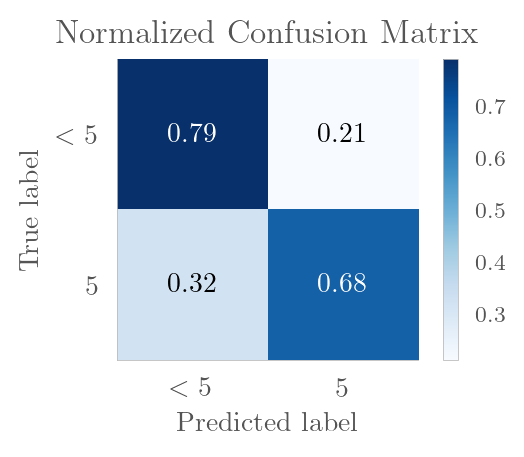
\includegraphics{Figures/logreg_l2_conf.png}
    \caption{Confusion matrix for binary classification using logistic 
    regression with $L_2$ penalization.}
    \label{fig:logreg_conf}
\end{figure}

The corresponding ROC-curve is shown in~\cref{fig:logreg_roc}. The curves for both classes are nearly identical, showing that class imbalances do not affect the
classification to a disastrous extent. 

\begin{figure}[H]
    \centering
    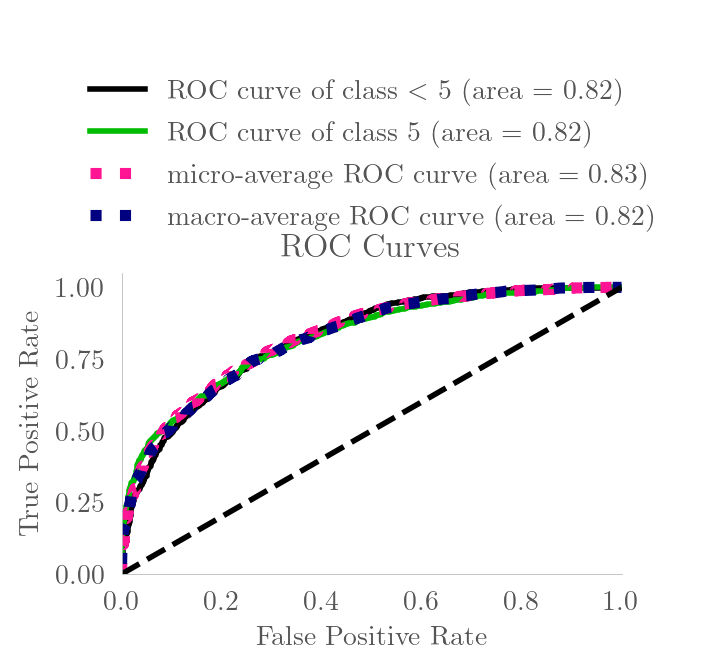
\includegraphics{Figures/logreg_l2_roc.png}
    \caption{The ROC curve for logistic regression with $L_2$ penalization.}
    \label{fig:logreg_roc}
\end{figure}

\subsection{Random Forest}

Random forests and other ensemble methods have many hyperparameters
available for tuning. To limit the scope, only the number of trees and the
maximum tree depth were explored. The error decomposition of each is shown
in~\cref{fig:randfor_err}. A bit surprisingly, random forest gives good results
even with few trees of small depth. As there are more than a 100 predictors,
this implies that many of them contain little information.

\begin{figure}[H]
    \centering
    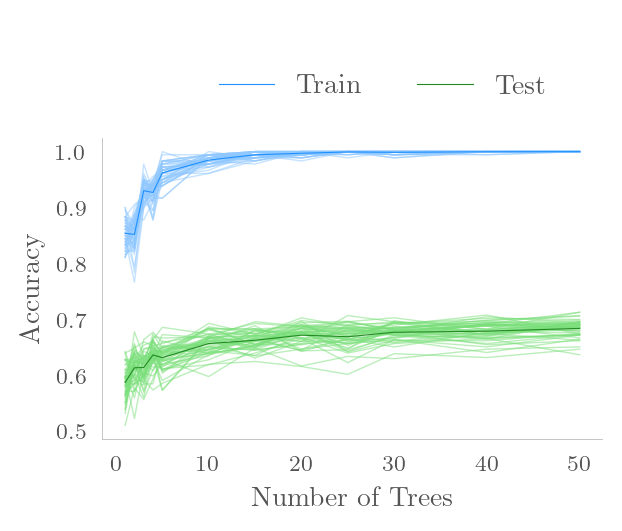
\includegraphics{Figures/randforest_bootstrap.png}
    \caption{The accuracy of random forest as a function of number of trees.
    Notice the perfect training accuracy.}
    \label{fig:randfor}
\end{figure}

\begin{figure}[H]
    \begin{subfigure}
        \centering
        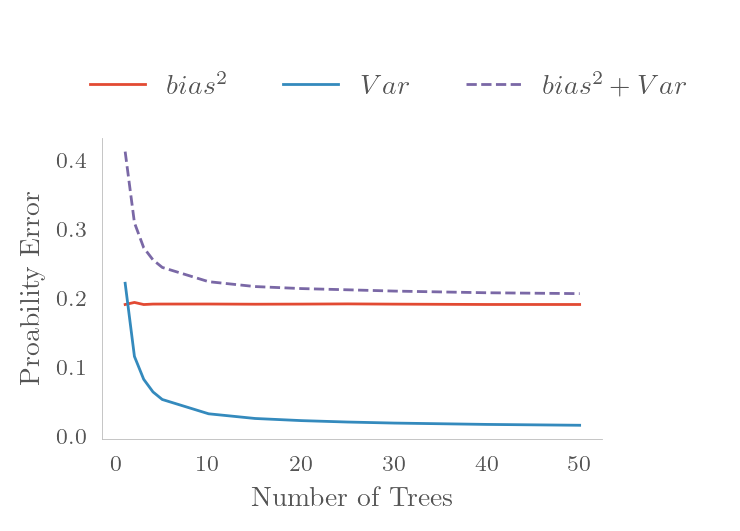
\includegraphics{Figures/randforest_biasvar.png}
        \caption{The error decomposition
        as function of number of trees. The depth is kept constant
        at 50.}
    \end{subfigure}
    \begin{subfigure}
        \centering
        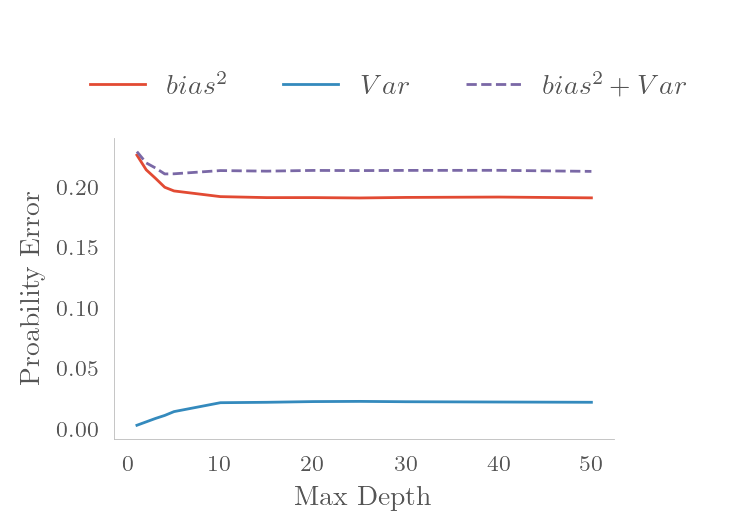
\includegraphics{Figures/randforest_depth_biasvar.png}
        \caption{The error decomposition
        as function of number of depth. The number of trees is kept
        constant at 20}
    \end{subfigure}
    \caption{Error decomposition by bootstrapping for random forests.}
    \label{fig:randfor_err}
\end{figure}

It is~\cref{fig:randfor} that is the most alarming, however. 
Once the number of trees gets sufficiently high, the training accuracy becomes
\textit{perfect}. This indicates either that the method overfits the training
set, or that the response is leaking into the predictors. As both the error decomposition and test accuracy does not deteriorate, overfitting is not the
culprit. The investigation of response leakage is postponed till~\cref{subsec:response_leakage}.

The resulting confusion matrix using the found optimal hyperparameters
is shown in~\cref{fig:randfor_conf}. It is nearly identical to logistic regression \cref{fig:logreg_conf}, being slightly better at $<5$ but worse at $5$. If our
suspicion of defaulting to $<5$ as discussed earlier is correct, it implies
than random forests performes worse than logistic regression. The associated
ROC curve is not shown as it is nearly identical to that of logistic regression.

\begin{figure}[H]
    \centering
    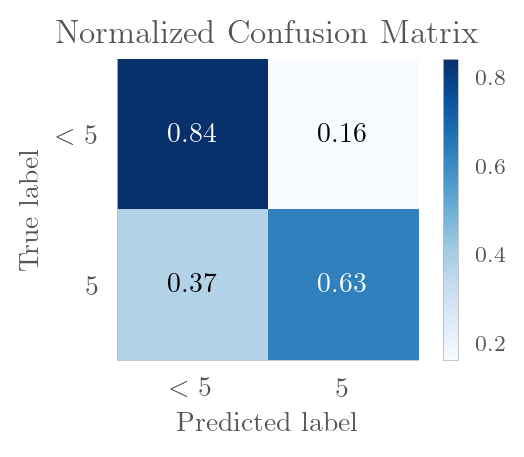
\includegraphics{Figures/randforest_conf.png}
    \caption{The confusion matrix for random forest.}
    \label{fig:randfor_conf}
\end{figure}

\subsection{AdaBoost}\label{subsec:adaboost}

Just like random forest, AdaBoost provides a plethora of tuneable
hyperparameters. The number of trees and learning rate were chosen, with
their error decomposition shown in~c\ref{fig:adaboost_err} and behavior of
accuracy as function of number of trees shown in~\cref{fig:ada_trees}. 
Neither hyperparameter give widely different performance, only slightly decreasing 
variance while slightly increasing bias. 

The behavior of the accuracy however, is markedly different from the earlier methods, requiring a large number of trees to give "good" training accuracy. More 
pointedly, the test and training accuracy start out equal[WHY] with the test accuracy reaching a maximum at just $4$ trees. In contrast to random trees, this
does not point to response leakage, but overfitting. 

\begin{figure}[H]
    \centering
    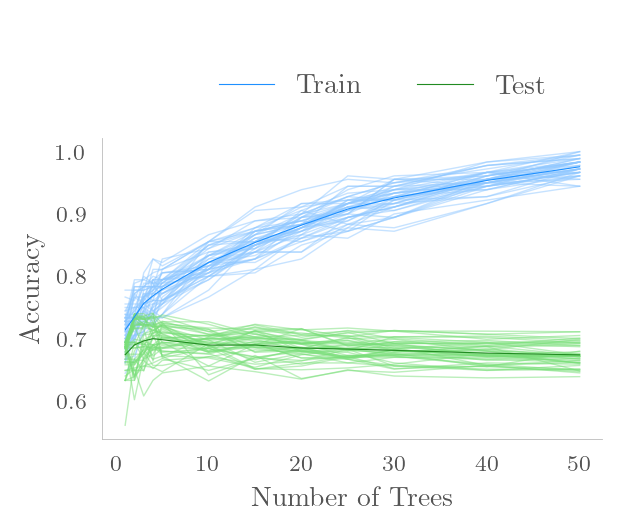
\includegraphics{Figures/ada_bootstrap.png}
    \caption{The accuracy of AdaBoost as a function of number of trees.
    Compare with the similar~\cref{fig:randfor}.}
    \label{fig:ada_trees}
\end{figure}

\begin{figure}[H]
    \begin{subfigure}
        \centering
        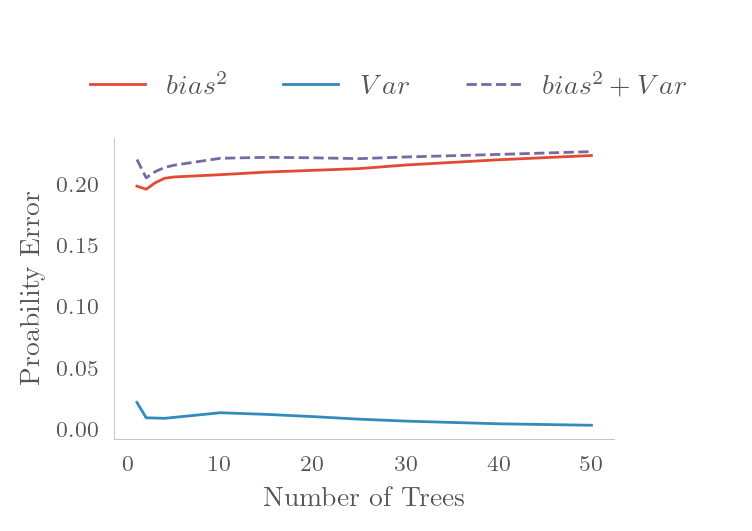
\includegraphics{Figures/ada_biasvar.png}
        \caption{The error decomposition
        as function of number of trees. The depth is kept constant
        at 50.}
    \end{subfigure}
    \begin{subfigure}
        \centering
        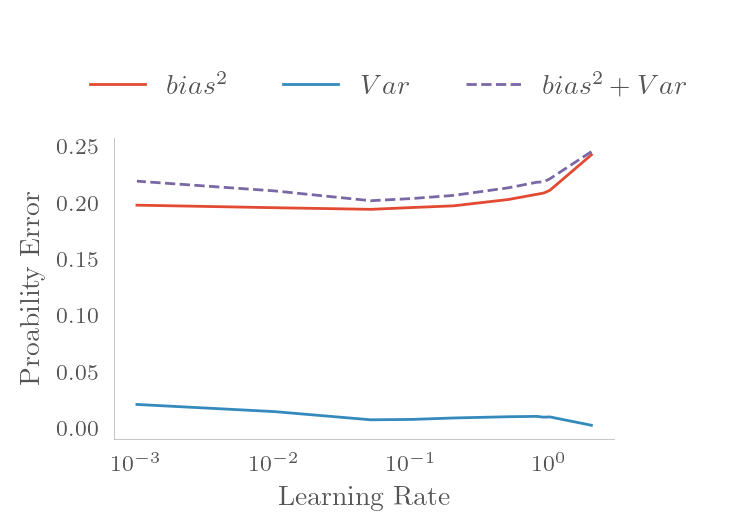
\includegraphics{Figures/ada_lr_biasvar.png}
        \caption{The error decomposition
        as function of learning rate. The number of trees is kept
        constant.}
    \end{subfigure}
    \caption{Error decomposition by bootstrapping using AdaBoost.}
    \label{fig:adaboost_err}
\end{figure}

As before, the confusion matrix for AdaBoost was created used the found
optimal hyperparameters. This is shown in~\cref{fig:adaboost_conf}. The results
are similar to and slightly better than random forest.

\begin{figure}[H]
    \centering
    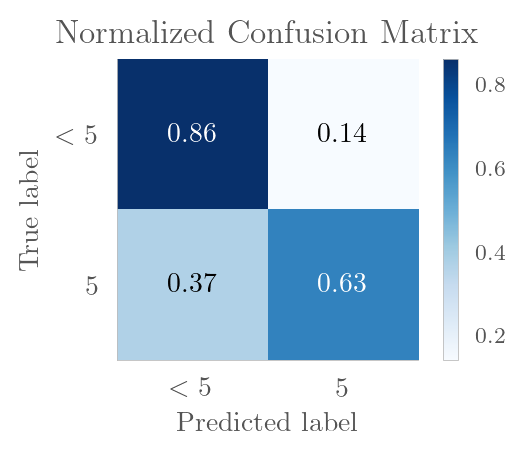
\includegraphics{Figures/ada_conf.png}
    \caption{The confusion matrix from using AdaBoost}
    \label{fig:adaboost_conf}
\end{figure}

\subsection{Response Leakage}\label{subsec:response_leakage}

To investigate the possibility of the response leaking into the features,
the random forest and AdaBoost models are used to extract the most important
features used by each. This is shown in~\cref{fig:featureselect}. Immediately the possible culprits reveal themselves. Both
methods rely heavily on \texttt{average stars}, describing the average number of stars given by the user, and \texttt{stars}, the average number of stars given
to the business. If the number of \texttt{average stars} and \texttt{stars} is 
large, there should be no response leakage due to the fact that there is no way to connect which observation of one corresponds to the other. However, if the number is small, they
would be highly predictive of the response simply because they \textit{equal} the
response. 

\begin{figure}[H]
    \begin{subfigure}
        \centering
        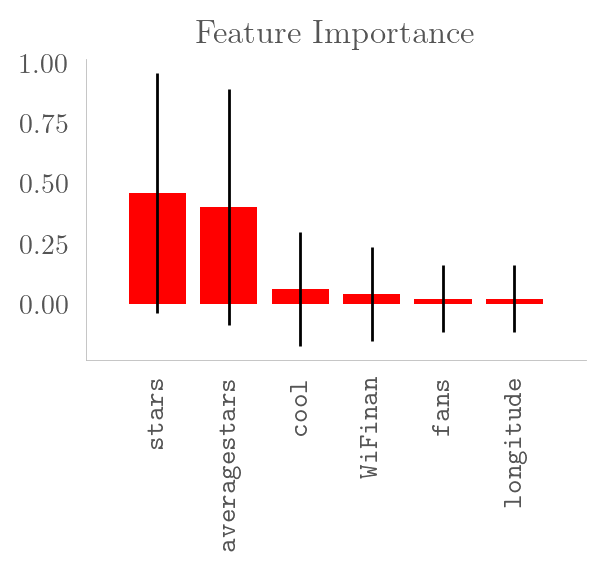
\includegraphics{Figures/ada_feature_importance.png}
        \caption{The features in the dataset ranked by importance by AdaBoost.
        All features not shown have been excluded by the method.}
    \end{subfigure}
    \begin{subfigure}
        \centering
        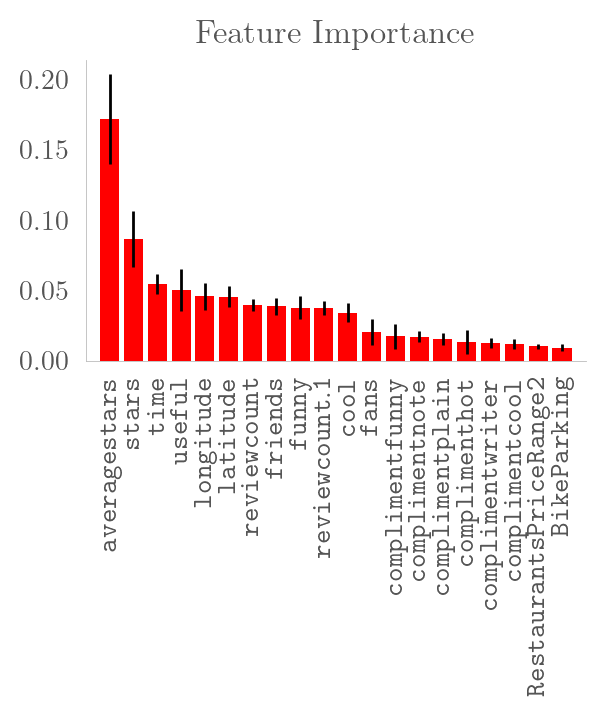
\includegraphics{Figures/randforest_feature_importance.png}
        \caption{The features in the dataset ranked by importance by random forest.}
    \end{subfigure}
    \label{fig:featureselect}
\end{figure}

To investigate the relationship between the mentioned features and the response
\texttt{rating}, they are plotted by violin plots in~\cref{fig:violin}. For all
values of \texttt{rating} there is significant spread in both \texttt{average stars} and \texttt{stars}, but also a clear correlation: users that give rating 1 to a business tends to give more 1s overall; vice versa for 5, and
slightly weaker for the other ratings. Interestingly rating 3 and 4 are centered around 3 and 4, suggesting
that users that give "ok" ratings are precisely those that tend to give "ok" ratings. The same goes for the \texttt{stars}: businesses that tend to get 5 stars are more likely to get more 5 stars. There is a weaker correlation between the other \texttt{stars} ratings. 

\begin{figure}[H]
    \begin{subfigure}
        \centering
        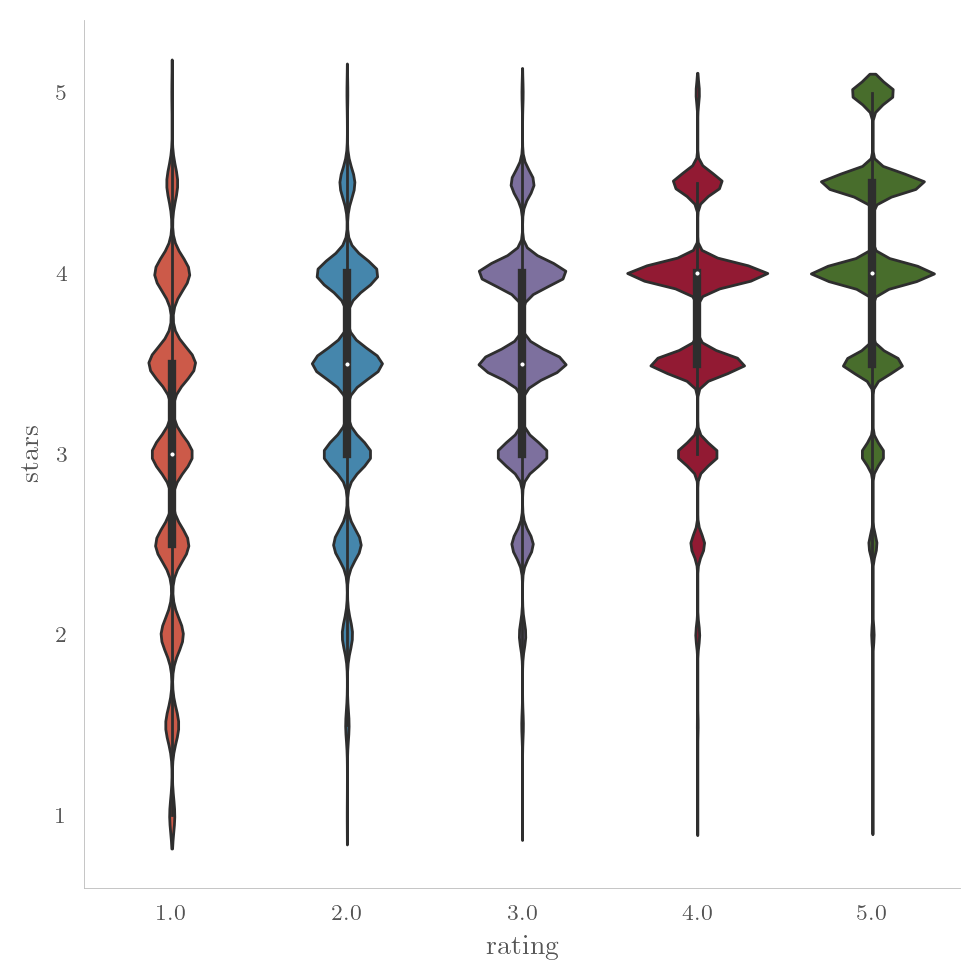
\includegraphics[width=\columnwidth]{Figures/rating_stars.png}
        \caption{The response \texttt{rating} plotted against
        \texttt{stars}, the average number of stars given to the business.}
    \end{subfigure}
    \begin{subfigure}
        \centering
        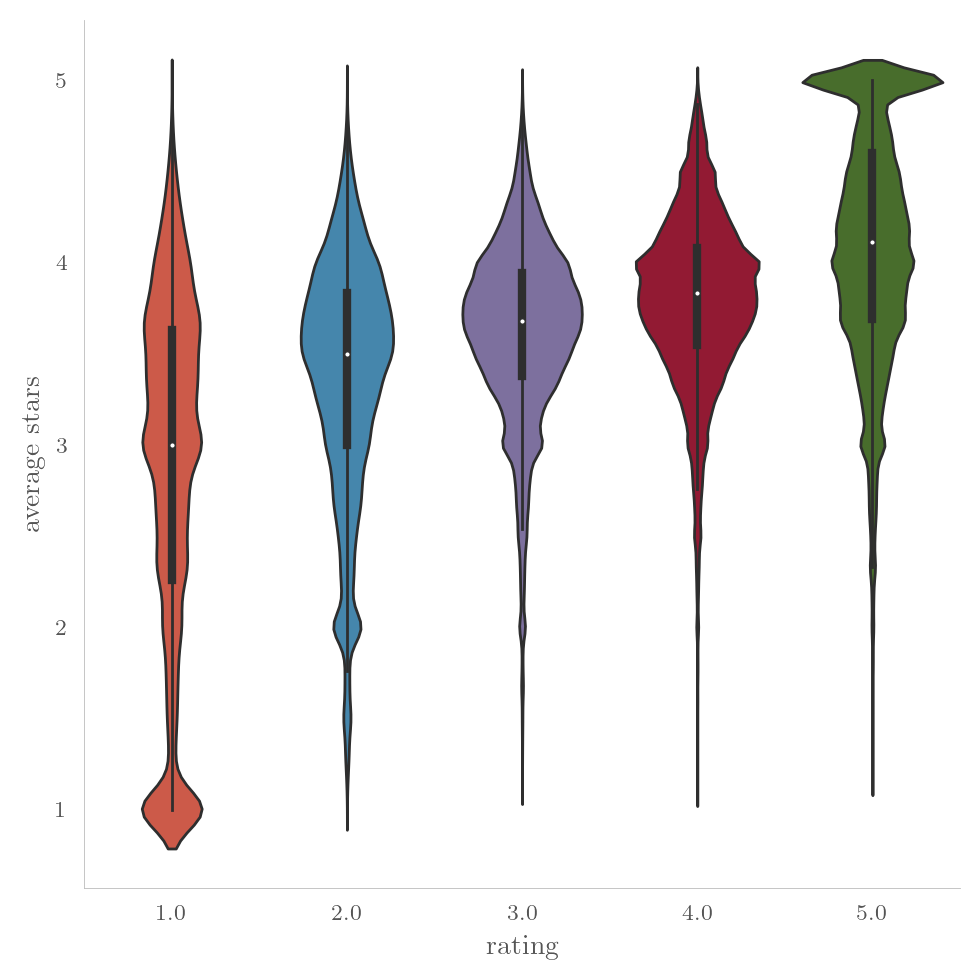
\includegraphics[width=\columnwidth]{Figures/av_stars.png}
        \caption{The response \texttt{rating} plotted against
        \texttt{average stars}, the average number of stars given by the user.}
    \end{subfigure}
    \label{fig:violin}
\end{figure}

In addition, there is reason to not be too worried about response leakage 
as AdaBoost relies much more on these two features than random forest, but
it is the random forest that gives perfect training accuracy while AdaBoost
gives similar accuracy for both training and test.


To summary, there is the possibility of the response leaking into the features, but this is not strongly
supported. The more likely explanation is a type of "rating inertia" for both businesses and users. Those businesses
that have generally high ratings are more likely to get more favorable reviews, and users that tend to give high ratings are more likely to give favorable reviews. An interesting question then becomes: what happens when \texttt{average stars} and \texttt{stars} are removed from the dataset?

\subsection{Hamstringing the Data}

To investigate the effect of \texttt{average stars} and \texttt{stars}, they were
removed from the dataset and the analysis was repeated. The results were very similar
across the methods, with the most important behavior summarized the confusion 
matrix in~\cref{fig:logregham}.
The classification of $<5$ is impressive, but alas, the classification of $5$ is abysmal, not better than chance. This supports our previous suspicion that the
algorithms defaults to $<5$, requiring unreasonable evidence to classify something 
as $5$. 

\begin{figure}[H]
    \centering
    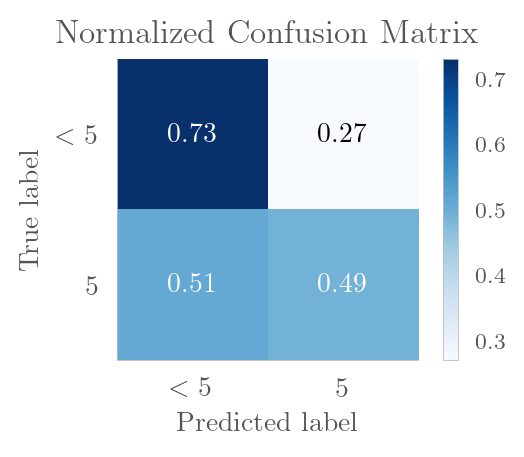
\includegraphics{Figures/logreg_l2_ham.png}
    \caption{The confusion matrix for Yelp data with \texttt{stars} and
    \texttt{average stars} removed. The class $5$ is nearly completely mislabeled.
    The method used was logistic regression with $L_2$ penalty. The ROC AUC was $0.62$.}
    \label{fig:logregham}
\end{figure}